\section{Results}
\label{chapter:results}
\subsection{Pre-processing}
To evaluate whether or not our graph reduction technique works, we have used nine different datasets. These datasets vary between 34 and well over a million vertexes. The amount of edges varies between 78 to almost 3 million edges. There's also a significant variety in the ratio between edges and vertexes. At the low end, the edges-to-vertexes ratio is around 1.3, while the highest ratio is above 20. Figure \ref{fig:datasets} gives an overview of the different datasets.

\begin{figure}[H]
\begin{center}
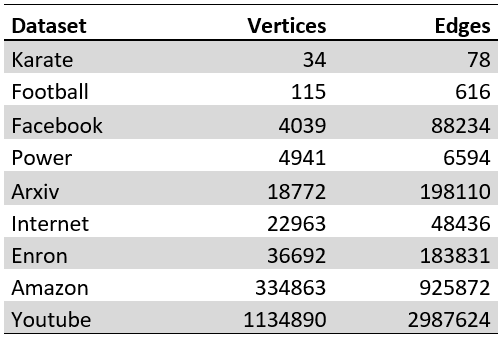
\includegraphics[width=0.5\textwidth]{images/datasets.png}
\caption{The variety of datasets used to test the algorithms}\label{fig:datasets}
\end{center}
\end{figure}

Figure \ref{fig:reducedtable} shows the results from the pre-processing algorithm. Since the algorithm uses random sampling, each graph was reduced five times and the results were averaged. The results were surprisingly good. Of the 9 graphs, 6 were reduced by around 30\% or more, while 3 were reduced by more than half both in nodes and in edges. The Internet and Power graphs did not see a lot of reduction. We believe this is due to the fact that they are graphs of internet relays and electricity relays respectively. These are inherently bound by geographic limitations, making it unlikely that large cliques form. For the YouTube dataset the reason is not immediately clear.

\begin{figure}[H]
\begin{center}
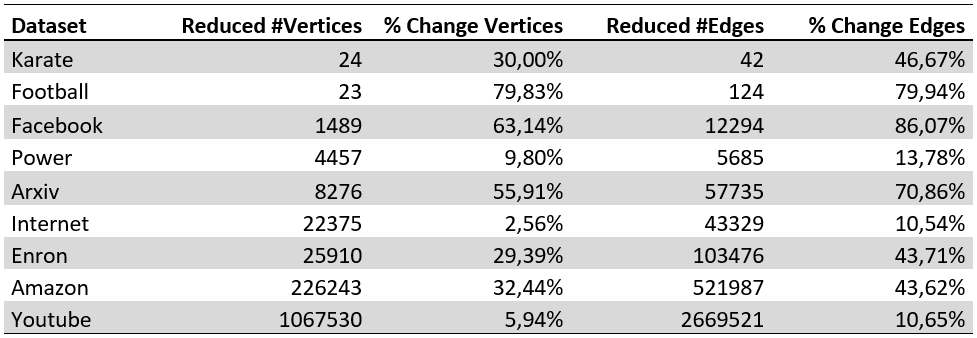
\includegraphics[width=1\textwidth]{images/reducedtable.png}
\caption{The amount of vertices and edges after the preprocessing step, as well as the percentage change.}\label{fig:reducedtable}
\end{center}
\end{figure}

The pre-processing algorithm is only useful if it doesn't take more time to run than the time it saves later on. After some iterating to solve performance issues, figure \ref{fig:prespeed} shows the average execution time to reduce each graph. The sampling method is clearly very fast, since even graphs with tens of thousands of vertexes can be processed in just a few seconds. Even the large YouTube dataset with over a million vertexes takes just under 10 minutes to process. These times are negligible compared to however long the community detection step will take on larger graphs. Another observation is that the graphs in which few cliques were found (Power and Internet) also take less time to process.

\begin{figure}[H]
\begin{center}
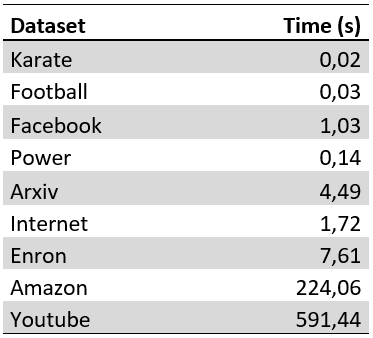
\includegraphics[width=0.4\textwidth]{images/prespeed.png}
\caption{The average execution time needed for the preprocessing step.}\label{fig:prespeed}
\end{center}
\end{figure}

\subsection{Community detection}
!!!TODO!!! algorithm settings !!!TODO!!!
To test the effects of reducing the graph, we ran the community detection genetic algorithm ten times for each graph, five times with the original graph and five times with a reduced graph. Execution time was limited to five minutes. The reported execution times and modularity scores are the averages of those five runs. The maximum execution time is only checked at the end of each generation, which is why the reported execution time can be significantly higher than five minutes. We have also noted the fitness score for a random community partitioning as a comparison. These are the average of 100 random partitionings for regular and reduced graphs. This provides a baseline measure to compare the results against.
\par
During testing we found that the self-learning operator took a very long time to complete compared to the other operators. This made generations take a very long time on larger graphs. Since we were mainly interested in the effects of reducing the graph, we disabled the self-learning operator for larger graphs. We have also repeated our tests for the smaller graphs without this operator. Results without the self-learning operator are marked with ``-SL''.\footnote{We believe this is mainly due to the slow initialization of the jenetics library. In the paper by Li and Liu, they do not seem to have this issue. }
\par
Even with the reduced graphs, the Amazon and YouTube graphs were still too large to solve in a reasonable amount of time. The Enron dataset was just barely possible, but we had to increase the maximum time to 10 minutes per run, and reduce the population size from 25 to 9.

\subsubsection{Karate}

\begin{figure}[H]
\begin{center}
    \begin{subfigure}{0.47\textwidth}
    \begin{center}
    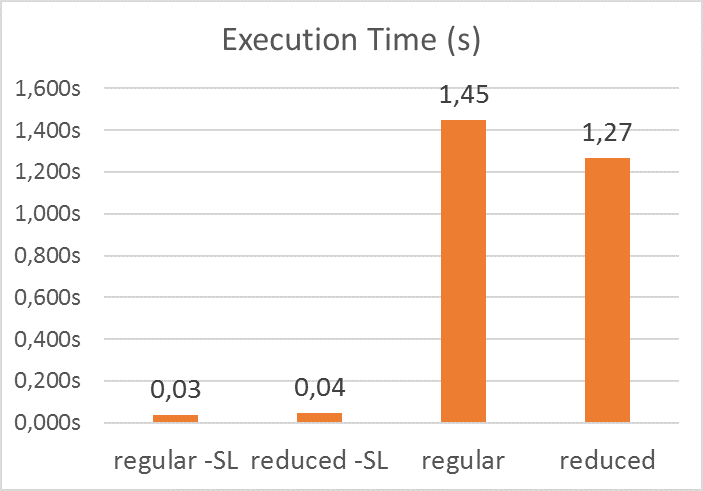
\includegraphics[height=5.4cm]{images/karatetime.png}
    \end{center}
    \end{subfigure}
    \begin{subfigure}{0.47\textwidth}
    \begin{center}
    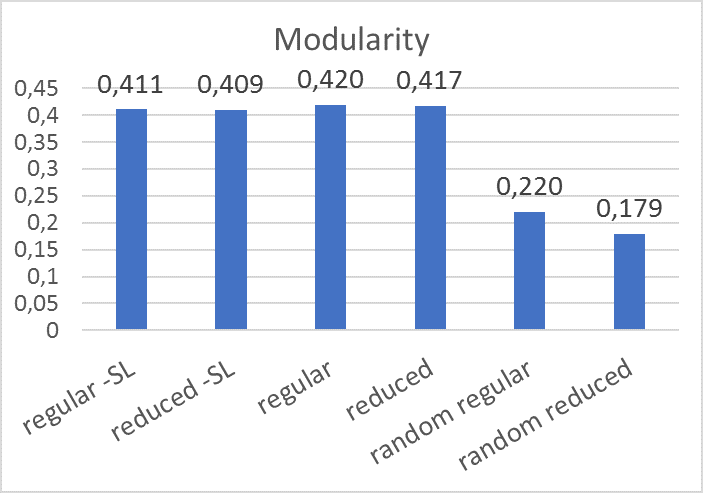
\includegraphics[height=5.4cm]{images/karatefitness.png}
    \end{center}
    \end{subfigure}
\caption{Results for the Karate graph}\label{fig:karate}
\end{center}
\end{figure}

The Karate graph is the smallest in the dataset. The reason why we have tested all the graphs with both the self-learning operator enabled and disable becomes immediatly clear, as the execution time goes from tens of milliseconds to seconds. However, we do see slightly better results in the modularity score with self-learning enabled. For this graph, reducing the graph seems to have a slightly negative effect. In all cases (including the random population average modularity), the reduced graph scores slightly worse than the regular graph. We expect this is due to the limited search space due to the reduction. In this small example, it is possible to properly explore the search space. We believe that the smallest cliques of size 3 may need to be split up for the best score.
\subsubsection{Football}
\begin{figure}[H]
\begin{center}
    \begin{subfigure}{0.47\textwidth}
    \begin{center}
    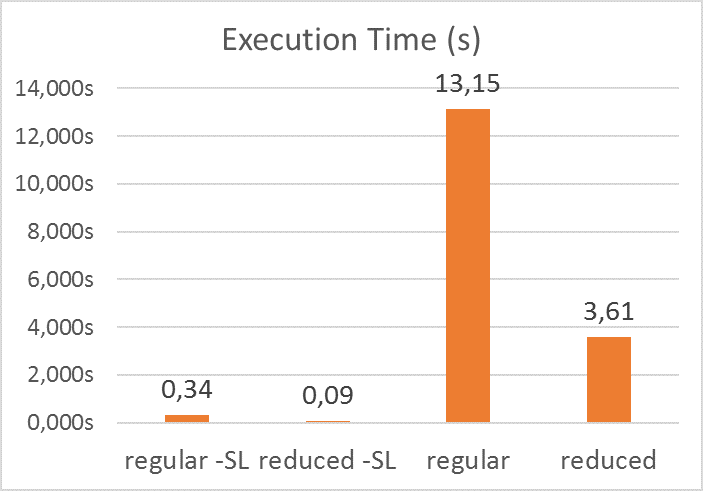
\includegraphics[height=5.4cm]{images/footballtime.png}
    \end{center}
    \end{subfigure}
    \begin{subfigure}{0.47\textwidth}
    \begin{center}
    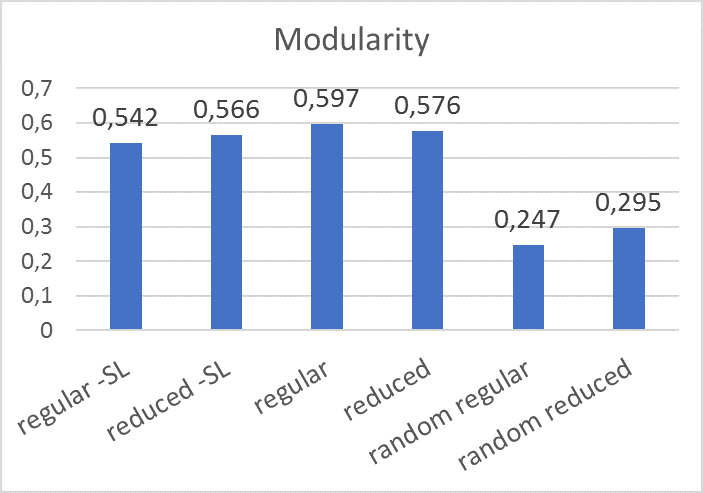
\includegraphics[height=5.4cm]{images/footballfitness.png}
    \end{center}
    \end{subfigure}
\caption{Results for the Football graph}\label{fig:football}
\end{center}
\end{figure}
The football graph is significantly larger and the advantages of reducing the graph are starting to show. The self-learning operator is still very slow, but no matter if it is enabled or disabled, the reduced graph significantly speeds up the algorithm. Without the self-learning operator we see a slight edge for the reduced graph, but with the operator enabled the edge goes back to the regular graph. With more than triple the execution time, the self-learning operator still manages to find a better solution than is possible with the reduced graph. The random scores give a signficant advantage to reduced graph. The football graph shows relations between players of several different football teams. Reducing parts of those teams to cliques makes sure that they stay together, even the communities are randomized, leading to the higher score.

\subsubsection{Facebook}
\begin{figure}[H]
\begin{center}
    \begin{subfigure}{0.47\textwidth}
    \begin{center}
    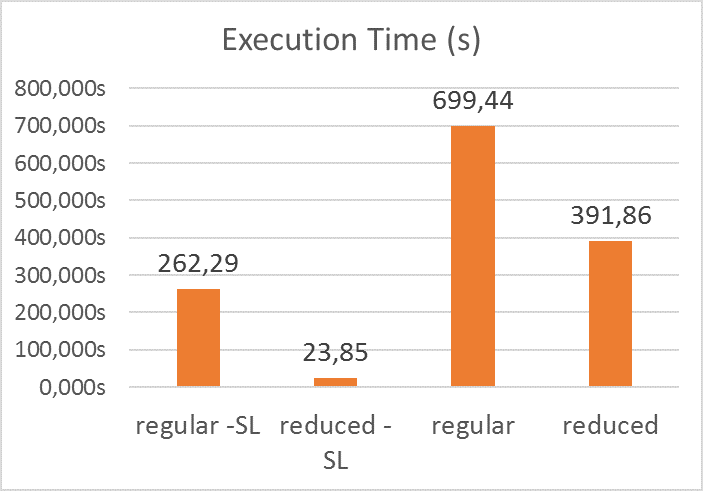
\includegraphics[height=5.4cm]{images/facebooktime.png}
    \end{center}
    \end{subfigure}
    \begin{subfigure}{0.47\textwidth}
    \begin{center}
    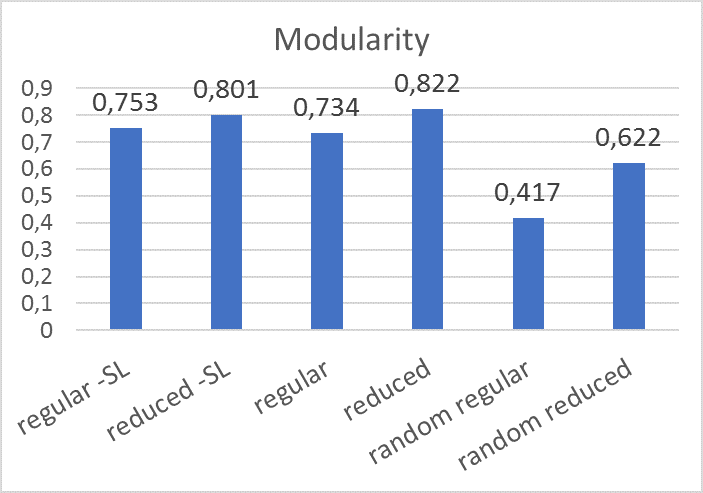
\includegraphics[height=5.4cm]{images/facebookfitness.png}
    \end{center}
    \end{subfigure}
\caption{Results for the Facebook graph}\label{fig:facebook}
\end{center}
\end{figure}
The Facebook graph is the best-case scenario for our algorithm. There are over 20 times as many edges as vertices, which left only around a third of the vertices and a sixth of the edges after reduction. There is a large lead in processing time for the reduced graph, and the scores are better across the board. Especially the random score is impressive: The random, initial population for the genetic algorithm is already significantly better with the reduced graph. The self-learning operator for the regular graph actually makes the score worse. The execution time got so high that only 2 or 3 generations can be processed. This is why we no longer include it in the larger graphs.

\subsubsection{Power}
\begin{figure}[H]
\begin{center}
    \begin{subfigure}{0.47\textwidth}
    \begin{center}
    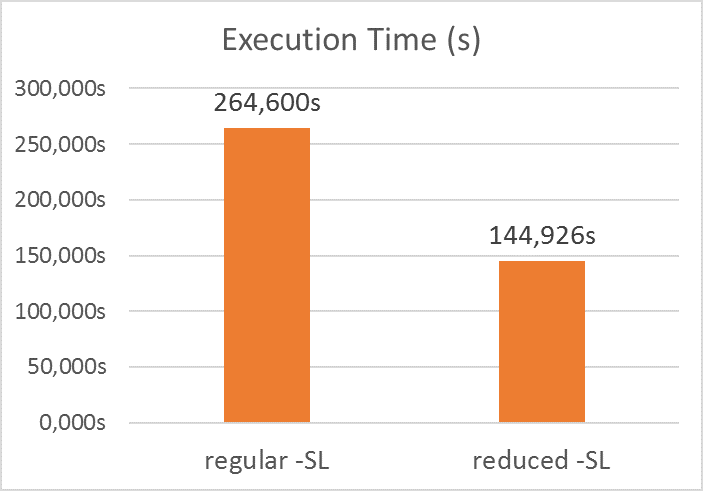
\includegraphics[height=5.4cm]{images/powertime.png}
    \end{center}
    \end{subfigure}
    \begin{subfigure}{0.47\textwidth}
    \begin{center}
    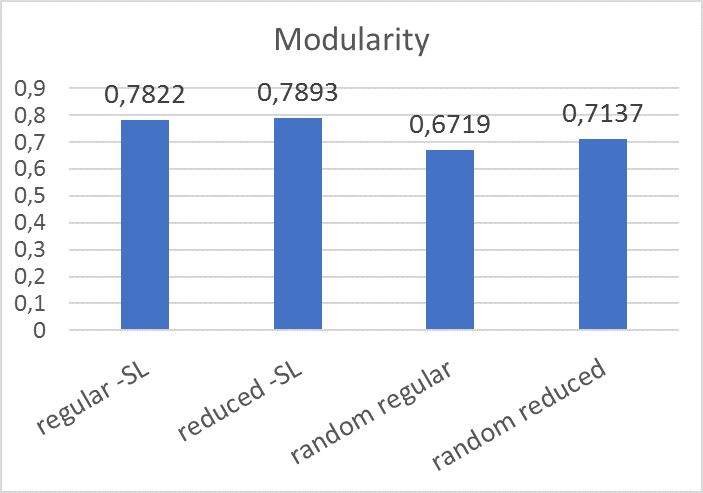
\includegraphics[height=5.4cm]{images/powerfitness.png}
    \end{center}
    \end{subfigure}
\caption{Results for the Power graph}\label{fig:power}
\end{center}
\end{figure}
The Power graph is a relatively bad case for our algorithm. The graph is only reduced by around 10\% of the vertices. However, there still is a large advantage for the reduced graph when it comes to execution time. The modularity of the 2 graphs is almost identical, but the random scores show a slight improvement for the reduced graph. For this graph, the reduction leads to a better start. This allows the algorithm to converge faster on roughly the same solution.

\subsubsection{Arxiv}
\begin{figure}[H]
\begin{center}
    \begin{subfigure}{0.47\textwidth}
    \begin{center}
    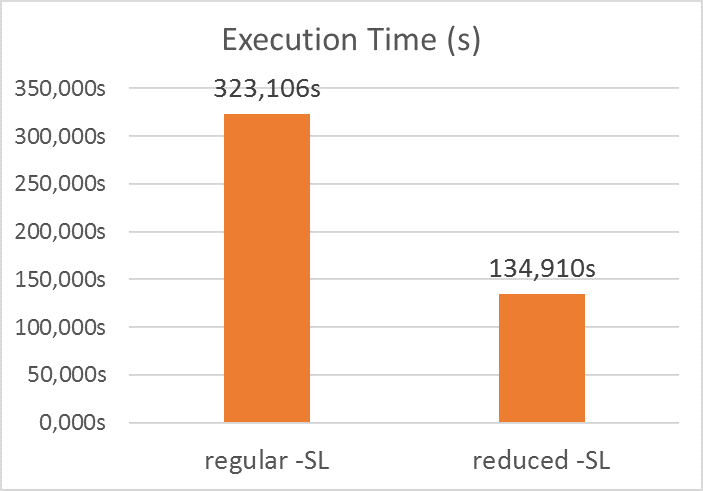
\includegraphics[height=5.4cm]{images/arxivtime.png}
    \end{center}
    \end{subfigure}
    \begin{subfigure}{0.47\textwidth}
    \begin{center}
    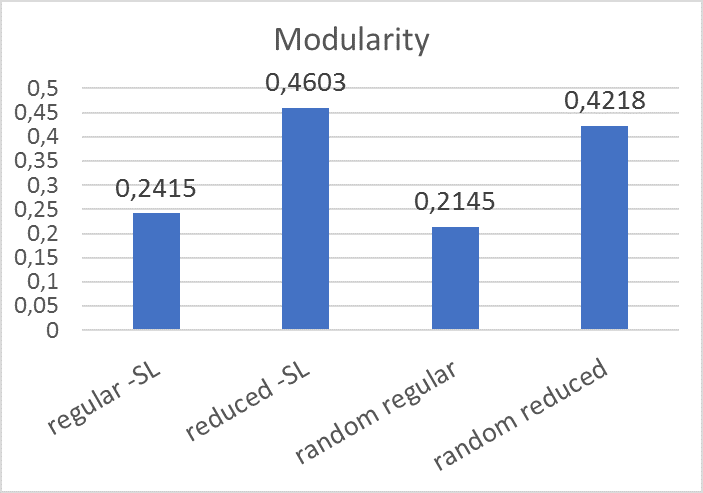
\includegraphics[height=5.4cm]{images/arxivfitness.png}
    \end{center}
    \end{subfigure}
\caption{Results for the Arxiv graph}\label{fig:arxiv}
\end{center}
\end{figure}
The Arxiv graph is another best-case example for the algorithm. There is a huge lead for the reduced graph both in execution time and score. However, most of the difference comes from the much better initial random population. The improvement on top of the baseline random score is roughly the same for both graphs. The effectiveness of the genetic algorithm is starting to suffer for graphs of this size.
\subsubsection{Internet}
\begin{figure}[H]
\begin{center}
    \begin{subfigure}{0.47\textwidth}
    \begin{center}
    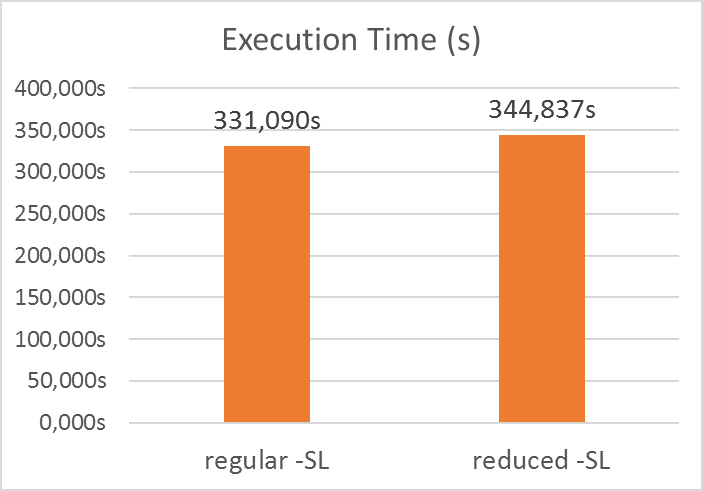
\includegraphics[height=5.4cm]{images/internettime.png}
    \end{center}
    \end{subfigure}
    \begin{subfigure}{0.47\textwidth}
    \begin{center}
    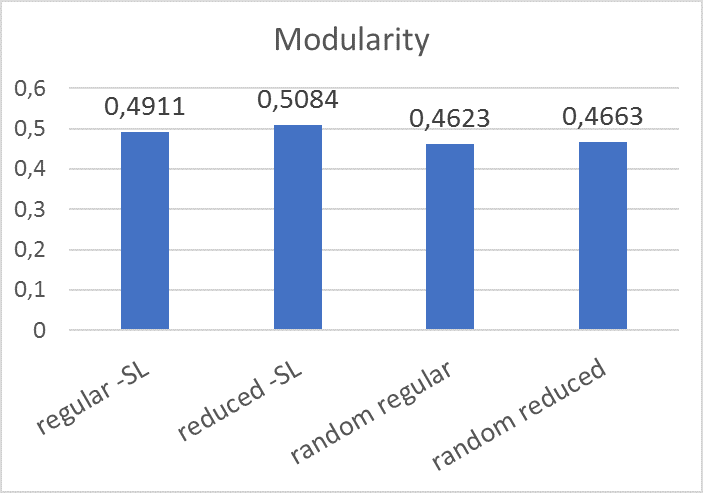
\includegraphics[height=5.4cm]{images/internetfitness.png}
    \end{center}
    \end{subfigure}
\caption{Results for the Internet graph}\label{fig:internet}
\end{center}
\end{figure}
The Internet graph could not be reduced much at all. Unsurprisingly, the results are almost identical. There is a slight modularity advantage for the reduced graph, but both scores are just slightly above the baseline score. The genetic algorithm is almost ineffective at this point.
\subsubsection{Enron}
\begin{figure}[H]
\begin{center}
    \begin{subfigure}{0.47\textwidth}
    \begin{center}
    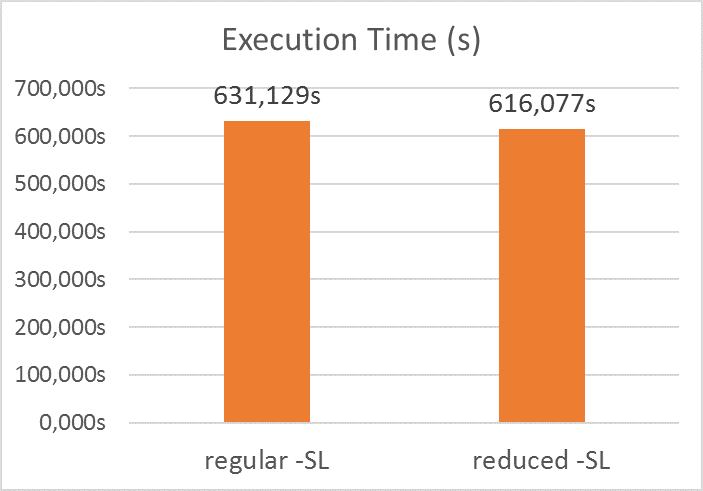
\includegraphics[height=5.4cm]{images/enrontime.png}
    \end{center}
    \end{subfigure}
    \begin{subfigure}{0.47\textwidth}
    \begin{center}
    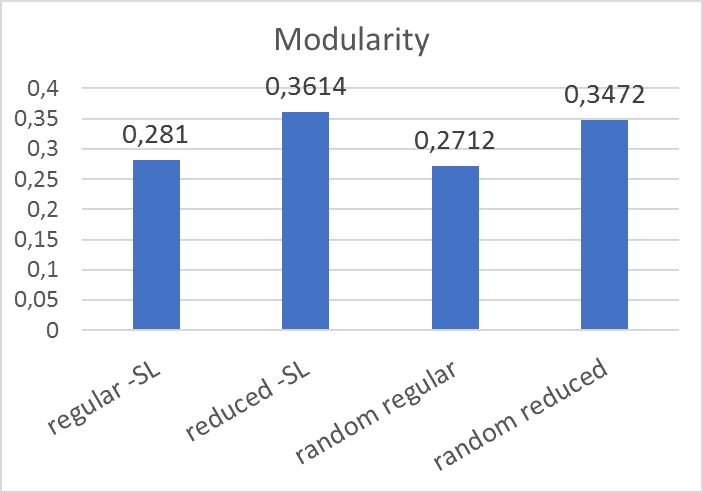
\includegraphics[height=5.4cm]{images/enronfitness.png}
    \end{center}
    \end{subfigure}
\caption{Results for the Enron graph}\label{fig:enron}
\end{center}
\end{figure}
The Enron graph is the largest graph we were able to process with the genetic algorithm, but we did give it a lower population size and twice the amount of time. The Enron graph could be reduced by about a third, and this expresses itself as an advantage in the random baseline score. The genetic algorithm just barely produces better results than the random baseline.

